\documentclass{beamer}
\usepackage[orientation=landscape,size=custom,width=15.11,height=8.5,scale=1,debug]{beamerposter} % width=11.333,height=8.5
\geometry{paperwidth=15.11in,paperheight=8.5in} % paperwidth=11.333in,paperheight=8.5in
%\usepackage{helvet}
\usepackage{tikz}
\usepackage{lmodern} % Load Latin Modern fonts
\usepackage{subcaption}
\usepackage{multirow}
\usepackage{booktabs}
\usepackage{graphicx} % for including graphics
\usepackage{multicol}
\usepackage[citestyle=authoryear, bibstyle=authoryear, sorting=nyt]{biblatex}
\addbibresource{../1_SOC_Honors.bib}
 
\usetheme{Madrid}

% Color settings
\setbeamercolor{normal text}{bg=white, fg=black}
\setbeamercolor{alerted text}{bg=white, fg=black}
\setbeamercolor{structure}{bg=white, fg=cyan!70}
%\setbeamercolor{navigation symbols}{bg=white, fg=white}
\setbeamercolor{title}{bg=cyan!7, fg=black}
\setbeamercolor{subtitle}{bg=white, fg=black}
\setbeamercolor{section in toc}{bg=white, fg=black}
\setbeamercolor{subsection in toc}{bg=white, fg=black}
\setbeamercolor{frametitle}{bg=cyan!7, fg=black}
\setbeamercolor{block title}{bg=white, fg=black}
\setbeamercolor{block title alerted}{bg=white, fg=black}
\setbeamercolor{block title example}{bg=white, fg=black}
\setbeamercolor{section number projected}{bg=white, fg=black}

% Header/Footer colors
\setbeamercolor{author in head/foot}{bg=cyan!7,fg=black} 
\setbeamercolor{title in head/foot}{bg=cyan!7,fg=black} 
\setbeamercolor{date in head/foot}{bg=cyan!7,fg=black} 
\setbeamercolor{page number in head/foot}{bg=cyan!7,fg=black}


% Redefine section in toc to include section numbers
\setbeamertemplate{section in toc}{\inserttocsectionnumber.~\inserttocsection}
\setbeamertemplate{navigation symbols}{}
%\setbeamertemplate{frametitle}[default][center]

\setbeamerfont{footnote}{size=\tiny}

% Redefine bibliography colors to black
\setbeamercolor{bibliography entry author}{fg=black}
\setbeamercolor{bibliography entry title}{fg=black} % Set book titles to black
\setbeamercolor{bibliography entry note}{fg=black}
\setbeamercolor{caption name}{fg=black}

\title[Construction Union\ldots{Historical-Comparative}]{Construction Union Agreements: Union Organizing in Historical-Comparative Perspective}
\author{Matthew Carson}
\date[Undergrad. Research Week '24]{Undergraduate Research Week 2024}

\begin{document}

\begin{frame}
  \titlepage
\end{frame}

%\begin{frame}{Table of Contents}
%  \begin{multicols}{2}
%    \tableofcontents
%  \end{multicols}
%\end{frame}

%%%%%%%%%%%%%%%%%%%%%%%%%%%%%
%                                                                                       %
%                                   Abstract                                       %
%                                                                                       %
%%%%%%%%%%%%%%%%%%%%%%%%%%%%%

% US Building Trade unions organize their workers differently. Most labor unions compel employers to negotiate, but the Building Trades engage in voluntary negotiations, relying on workers' skill levels rather than strike leverage. This approach correlates with their frequent political deviations from the broader US labor movement, particularly in opposing progressive environmental policies aligning more closely with the petrochemical industry on environmental issues and not supporting single-payer healthcare. One view is that unions pursue their members’ interests narrowly, sacrificing broader working-class interests if they feel it is necessary to secure work for their members, and some suggest that the conservative stance of the Building Trades stems from their craft union tradition, in which workers are organized by craft and skill instead of by industry. However, using historical-comparative methods, I show that these arguments do not hold. Petrochemical unions have supported progressive policies, and other craft-based unions have endorsed single-payer healthcare. However, unlike the Building Trades, those unions have never used voluntary agreements. Consequently, they have experienced more conflicts with employers. These findings challenge traditional views and suggest that the Building Trades' conservative negotiation strategies significantly shape their political and policy positions, reinforcing an employer-union dynamic that limits challenging management.

%%%%%%%%%%%%%%%%%%%%%%%%%%%%%
%%%%%%%%%%%%%%%%%%%%%%%%%%%%%

\section*{Introduction}
\begin{frame}{Introduction}
\textbf{Do the ways that unions organize affect their political stances?}\newline\newline % and how solidaristic they are with progressive movements?}\newline\newline
%US Building Trade unions organize their workers differently. 
Most labor unions compel employers to negotiate, \textit{\textbf{but the Building Trades engage in voluntary negotiations}}, relying on workers' skill levels rather than strike leverage. 
	\newline\newline
	\textbf{Building Trades (BT) are frequently political outliers.}
	\begin{itemize}
		\item Oppose progressive environmental policies that other unions have endorsed.
		\begin{itemize}
			\item Align more closely with the petrochemical industry (e.g., pipelines).
		\end{itemize}
		\item Do not support single-payer healthcare.
		\begin{itemize}
			\item Fifteen unions are Labor for Single-Payer Healthcare affiliates. None are building trades unions.
		\end{itemize}
	\end{itemize}
	
	%This approach correlates with their frequent political deviations from the broader US labor movement, particularly in opposing progressive environmental policies aligning more closely with the petrochemical industry on environmental issues and not supporting single-payer healthcare.
\end{frame}

\section*{Methods: Historical}

\begin{frame}{Methods: Historical}

\setlength{\arrayrulewidth}{0.0pt} % Set the thickness of the rules to 0
\begin{tabular}{|p{0.35\textwidth}|p{0.4\textwidth}|}
\hline
%\begin{minipage}[t][0.2\textheight][t]{\linewidth}
\textbf{Historical:}\newline
\textbf{Within-Case Analysis}\footfullcite{langeComparativeHistoricalMethods2013}
%\end{minipage}
&
\begin{itemize}
    \item Historical trajectory of the union.
    \item Durability: institutional arrangements.
    \item Structural features \& constraints.
    \item Institutional changes (mergers, etc.).
    \item Evolutionary or generative approach.\footfullcite{reedBoisAmericanPolitical1997}
\end{itemize}
\\
\hline
%\begin{minipage}[c][0.2\textheight][b]{\linewidth}
\textbf{Comparative:}\newline
\textbf{Between-Case Analysis}\footcite{langeComparativeHistoricalMethods2013}
%\end{minipage}
&
\begin{itemize}
    \item Differences in institutional features.
    \item Difference in political outcomes.
\end{itemize}
\\
\hline
\end{tabular}
\end{frame}


\begin{frame}{Case Selection\footnote{Image sources: UA Local 189, \url{https://images.app.goo.gl/XZJ2Es3X4TYtJqzP7}. OCAW, \url{https://web.archive.org/web/20010825164515im_/http://webshells.com/ocaw/555.gif}. USW, \url{https://images.app.goo.gl/e4s1xJdefhUXT6CK8}. IAM 751, \url{https://images.app.goo.gl/Bv4FR6ugSFoq6mb37}.}}
\begin{figure}
\begin{tikzpicture}[remember picture,overlay]
\node[anchor=north west,inner sep=0pt,yshift=-3cm,xshift=5cm] at (current page.north west) {
\begin{subfigure}[t]{0.2\linewidth}
  \centering 
  
\includegraphics[height=100pt]{IAM_751}
\end{subfigure}
\begin{subfigure}[t]{0.2\linewidth}
  \centering
  
\includegraphics[height=100pt]{UA_189}
\end{subfigure}%
\begin{subfigure}[t]{0.2\linewidth}
  \centering
  
\includegraphics[height=100pt]{OCAW}
\end{subfigure}
\begin{subfigure}[t]{0.2\linewidth}
  \centering
  
\includegraphics[height=100pt]{USW}
\end{subfigure}};
\end{tikzpicture}
\end{figure}

\vfill

\begin{itemize}
    \item \textbf{IAM}\footfullcite{mccannBloodWaterHistory1989}: International Association of Machinists District 751
    \item \textbf{UA}\footfullcite{schneirovPrideSolidarityHistory1993}: United Association of Plumbers and Pipefitters Local 189
    \item \textbf{OCAW/USW}\footfullcite{leopoldManWhoHated2007}: Oil Chemical and Atomic Workers Union (now part of the United Steelworkers)
\end{itemize}
\end{frame}


\begin{frame}{Case Selection Table}
\begin{figure}
\begin{tikzpicture}[remember picture,overlay]
\node[anchor=north west,inner sep=0pt,yshift=-3cm,xshift=5cm] at (current page.north west) {
\begin{subfigure}[t]{0.2\linewidth}
  \centering 
  
\includegraphics[height=100pt]{IAM_751}
\end{subfigure}
\begin{subfigure}[t]{0.2\linewidth}
  \centering
  
\includegraphics[height=100pt]{UA_189}
\end{subfigure}%
\begin{subfigure}[t]{0.2\linewidth}
  \centering
  
\includegraphics[height=100pt]{OCAW}
\end{subfigure}
\begin{subfigure}[t]{0.2\linewidth}
  \centering
  
\includegraphics[height=100pt]{USW}
\end{subfigure}};
\end{tikzpicture}
\end{figure}

\vfill

\begin{table}[]
    \centering
    \fontsize{17}{14}\selectfont
    \begin{tabular}{@{}llll@{}}
        \toprule
        \textbf{Union} & \textbf{Similarity} & \textbf{Difference} & \textbf{Outcome} \\ 
        \midrule[0.25pt] \midrule[0.25pt]
        Machinists (IAM) & \multirow{2}{*}{\begin{tabular}[c]{@{}l@{}}Both\\ craft\\ unions\end{tabular}} & \begin{tabular}[c]{@{}l@{}}•Industrial mode of organizing\\ •Involuntary agreements\end{tabular} & •Support progressive social-wage policy (e.g., single-payer healthcare). \\ 
        \cmidrule(r){1-1} \cmidrule(l){3-4} 
        Plumbers/Pipefitters (UA) & & •Voluntary agreements & •No/limited support for social-wage policy. \\ 
        \midrule[0.25pt] \midrule[0.25pt]
        \begin{tabular}[c]{@{}l@{}}Oil Chemical \& Atomic\\ Workers/Steelworkers\\ (OCAW/USW)\end{tabular} & \multirow{2}{*}{\begin{tabular}[c]{@{}l@{}}Both \\ have \\ substantial \\ petrochemical \\ work\end{tabular}} & \begin{tabular}[c]{@{}l@{}}•Industrial mode of organizing\\ •Involuntary agreements\end{tabular} & \begin{tabular}[c]{@{}l@{}}•Supports progressive social-wage policy.\\•Supports the Pollan Report---creation of clean-energy jobs\\and a transition from fossil fuels.\end{tabular} \\ 
        \cmidrule(r){1-1} \cmidrule(l){3-4} 
        Plumbers/Pipefitters (UA) & & •Voluntary Agreements & \begin{tabular}[c]{@{}l@{}}•No/limited support for social-wage policy.\\•Has defended the construction of new oil pipelines.\\•Opposed reforms and regulatory policies that might\\hamper new refinery projects\end{tabular} \\ 
        \bottomrule
    \end{tabular}
    \caption{The most similar cases that had different outcomes were selected.}
    \label{tab:my-table}
\end{table}
\end{frame}



\section*{Union Organizing Paths}
%\subsection*{NLRB Election}
%\begin{frame}{Union Organizing Paths: NLRB Election}
%  \begin{columns}
%    \column{0.725\textwidth}
%    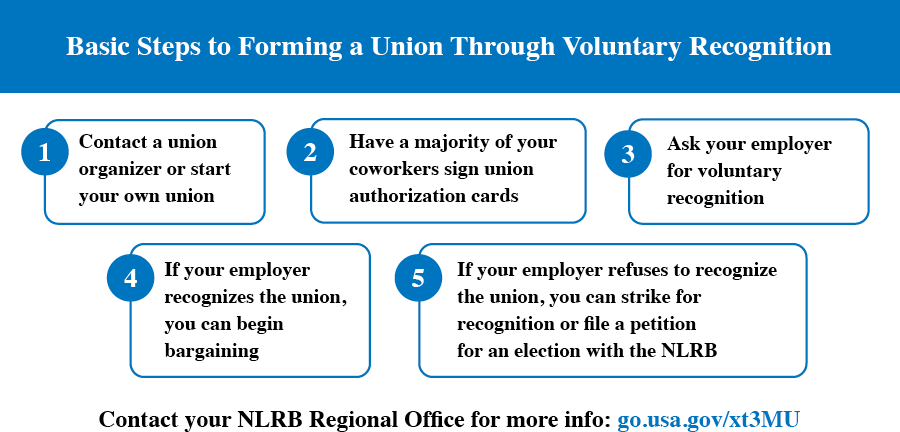
\includegraphics[width=0.9\linewidth]{../images/DOL}
%    \begin{scriptsize}
%	    \begin{center}
%	    	(Source: US Department of Labor.)
%	    \end{center}    
%    \end{scriptsize}
%    
%    
%    \column{0.275\textwidth}
%     Designed for the \underline{industrial unions} forming at the time of the passage of the National Labor Relations Act.
%    \newline\newline
%    However, it was not designed for the Building Trades because they were already organizing differently.
%
%    \end{columns}
%\end{frame}

\subsection*{Comparison}

\begin{frame}{Union Organizing Paths: Comparison} %\footfullcite{dolWORKCenterUnions, nlrbNLRBProcess}}
  \begin{columns}
    \column{0.6\textwidth}
    \includegraphics[scale=0.148]{../images/organizing_paths_2}

    \column{0.4\textwidth}
    The industrial mode of organizing (left) and the construction mode of organizing (right).\newline\newline
    Construction unions may follow either path, but other unions may not voluntarily negotiate the way that construction unions can.
    \end{columns}
\end{frame}

\begin{frame}{Union Organizing Paths: Comparison} %\footfullcite{dolWORKCenterUnions, nlrbNLRBProcess}}
  \begin{columns}
    \column{0.6\textwidth}
    \includegraphics[scale=0.148]{../images/organizing_paths_3}

    \column{0.4\textwidth}
    The industrial mode of organizing (left) and the construction mode of organizing (right).\newline\newline
    Construction unions may follow either path, but other unions may not voluntarily negotiate the way that construction unions can.
    \end{columns}
\end{frame}

\begin{frame}{Union Organizing Paths: Comparison} %\footfullcite{dolWORKCenterUnions, nlrbNLRBProcess}}
  \begin{columns}
    \column{0.6\textwidth}
    \includegraphics[scale=0.148]{../images/organizing_paths_4}

    \column{0.4\textwidth}
    The industrial mode of organizing (left) and the construction mode of organizing (right).\newline\newline
    Construction unions may follow either path, but other unions may not voluntarily negotiate the way that construction unions can.
    \end{columns}
\end{frame}

\begin{frame}{Union Organizing Paths: Comparison} %\footfullcite{dolWORKCenterUnions, nlrbNLRBProcess}}
  \begin{columns}
    \column{0.6\textwidth}
    \includegraphics[scale=0.148]{../images/organizing_paths_5}

    \column{0.4\textwidth}
    The industrial mode of organizing (left) and the construction mode of organizing (right).\newline\newline
    Construction unions may follow either path, but other unions may not voluntarily negotiate the way that construction unions can.
    \end{columns}
\end{frame}

\begin{frame}{Union Organizing Paths: Comparison} %\footfullcite{dolWORKCenterUnions, nlrbNLRBProcess}}
  \begin{columns}
    \column{0.6\textwidth}
    \includegraphics[scale=0.148]{../images/organizing_paths_7}

    \column{0.4\textwidth}
    The industrial mode of organizing (left) and the construction mode of organizing (right).\newline\newline
    Construction unions may follow either path, but other unions may not voluntarily negotiate the way that construction unions can.
    \end{columns}
\end{frame}

\begin{frame}{Union Organizing Paths: Comparison} %\footfullcite{dolWORKCenterUnions, nlrbNLRBProcess}}
  \begin{columns}
    \column{0.6\textwidth}
    \includegraphics[scale=0.148]{../images/organizing_paths_8}

    \column{0.4\textwidth}
    The industrial mode of organizing (left) and the construction mode of organizing (right).\newline\newline
    Construction unions may follow either path, but other unions may not voluntarily negotiate the way that construction unions can.
    \end{columns}
\end{frame}

\begin{frame}{Union Organizing Paths: Comparison} %\footfullcite{dolWORKCenterUnions, nlrbNLRBProcess}}
  \begin{columns}
    \column{0.6\textwidth}
    \includegraphics[scale=0.148]{../images/organizing_paths_9}

    \column{0.4\textwidth}
    The industrial mode of organizing (left) and the construction mode of organizing (right).\newline\newline
    Construction unions may follow either path, but other unions may not voluntarily negotiate the way that construction unions can.
    \end{columns}
\end{frame}

\begin{frame}{Union Organizing Paths: Comparison} %\footfullcite{dolWORKCenterUnions, nlrbNLRBProcess}}
  \begin{columns}
    \column{0.6\textwidth}
    \includegraphics[scale=0.148]{../images/organizing_paths_10}

    \column{0.4\textwidth}
    The industrial mode of organizing (left) and the construction mode of organizing (right).\newline\newline
    Construction unions may follow either path, but other unions may not voluntarily negotiate the way that construction unions can.
    \end{columns}
\end{frame}

\begin{frame}{Union Organizing Paths: Comparison}
  \begin{columns}
    \column{0.6\textwidth}
    \includegraphics[scale=0.148]{../images/organizing_paths}

    \column{0.4\textwidth}
    The industrial mode of organizing (left) and the construction mode of organizing (right).\footfullcite{dolWORKCenterUnions, nlrbNLRBProcess}\newline\newline
    Construction unions may follow either path, but other unions may not voluntarily negotiate the way that construction unions can.
    \end{columns}
\end{frame}

%\section{Building Trades Leverage}
%\begin{frame}{Building Trades Leverage}
%  \begin{columns}
%    \column{0.725\textwidth}
%    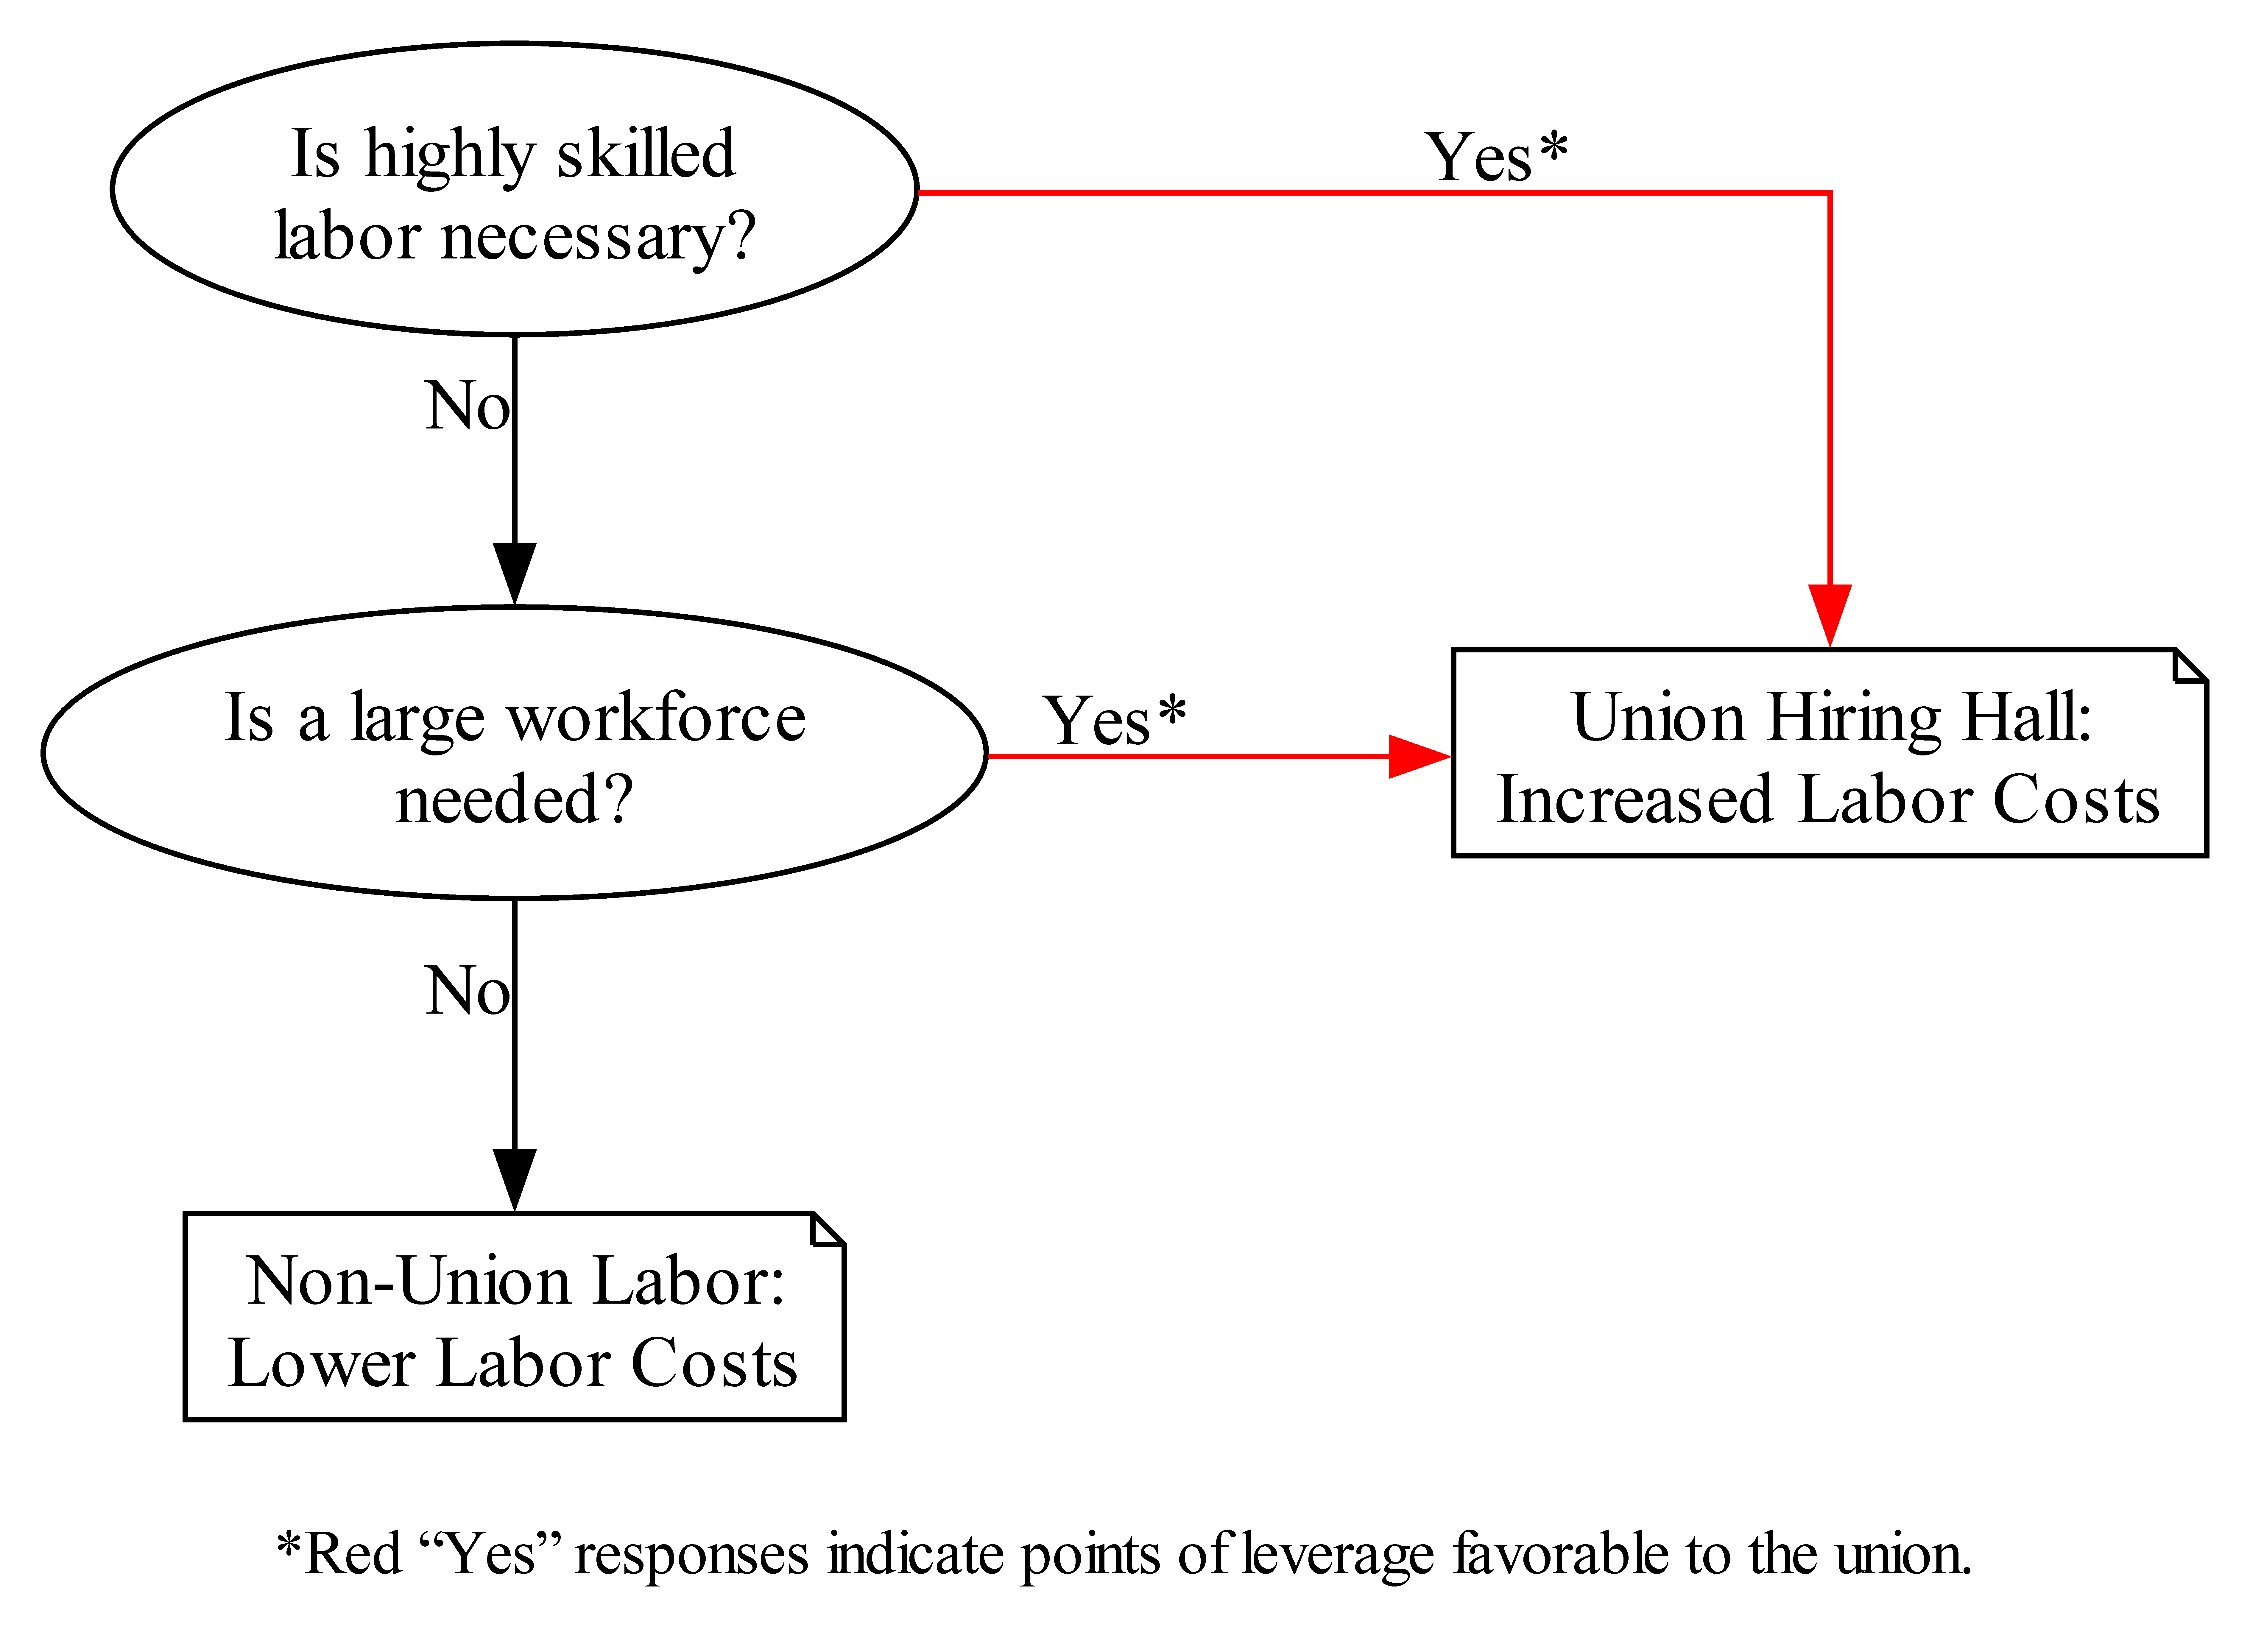
\includegraphics[width=\linewidth]{../images/union_power_red}
%
%    \column{0.275\textwidth}
%    Construction unions have more leverage when the employer requires a more skilled workforce or when the job is large and requires many employees.
%  \end{columns}
%\end{frame}

%\section{Building Trades Hiring Hall}
%\begin{frame}{Building Trades Hiring Hall}
%	\begin{columns}
%	\column{0.725\textwidth}
%	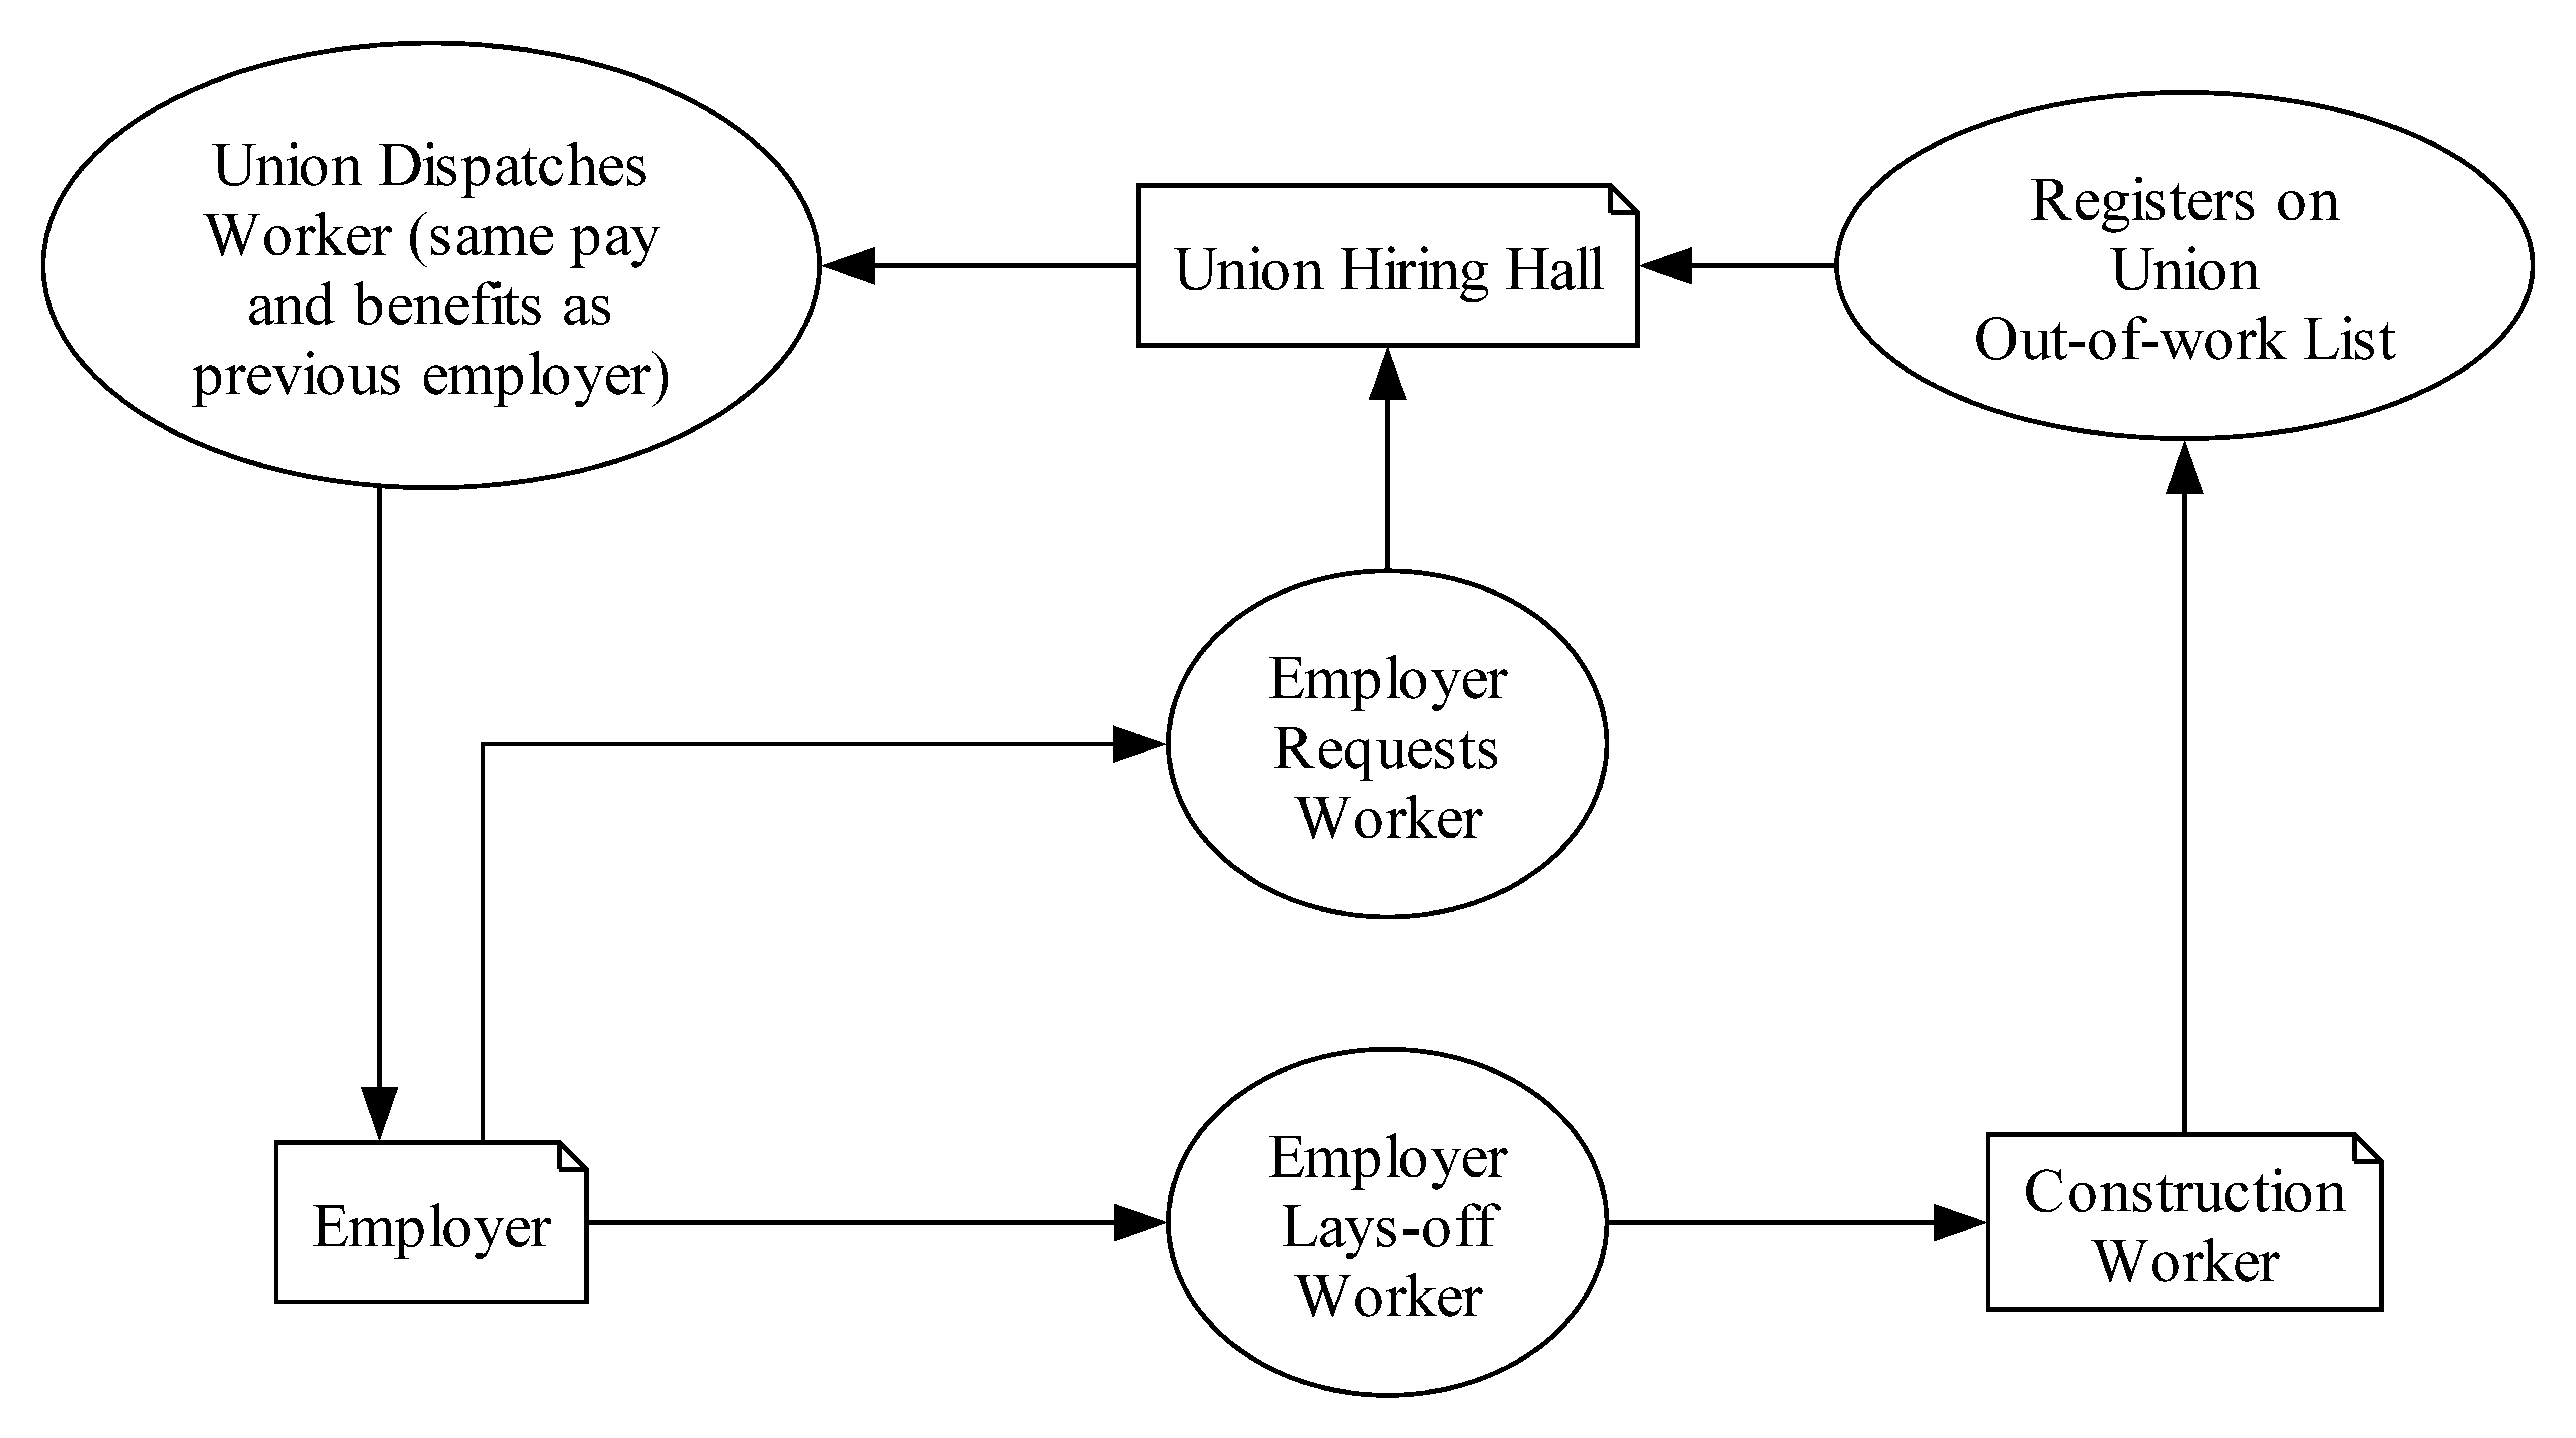
\includegraphics[width=\linewidth]{../images/hiring_hall}
%	\column{0.275\textwidth}
%	When employers require more workers for their projects, they contact the hiring hall to request workers to be dispatched to the job site.
%	\end{columns}
%\end{frame}

\section*{OCAW/USW vs. UA}
\begin{frame}{OCAW/USW vs. UA}
\textbf{Do unions align politically with the industry they work in?}\newline
\textbf{Do unions with petrochemical work align politically with the petrochemical industry?}\newline

\emph{Not necessarily.}
	\begin{itemize}
		\item The UA and OCAW/USW have taken very different political stances regarding clean energy transition.
		\item OCAW/USW has embraced a ``Just Transition" from dirty to clean energy.\footfullcite{leopoldManWhoHated2007}
	\begin{itemize}
		\item ``Just Transition": workers affected by the closure of plants, refineries, etc. are offered a safety net while transitioning to another career.
	\end{itemize}
	\item The United Association (UA) of Plumbers and Pipefitters (Building Trades) supports petrochemical industry-friendly policies.\footfullcite{natgasnowNextInfrastructureChallenge2015}
	\end{itemize}
The UA \textit{\textbf{does}} use pre-hire agreements, while the OCAW/USW \textbf{\textit{does not}}.
\end{frame}

\subsection*{Institutional consolidation}
\begin{frame}{OCAW/USW vs. UA}
\textbf{What explains why these unions organize differently?}\newline\newline
\underline{\textbf{Institutional}}
	\begin{itemize}
		\item United Association (UA)
			\begin{itemize}
				\item Apprenticeship and training as a ``bargaining chip."
				\item Prehire agreements are the norm.
				\item Institutional/structural features shaped the mode of organizing that the BT adopted.\footfullcite{schneirovPrideSolidarityHistory1993}
				\begin{itemize}
					\item They could have chosen a different mode.
					\item They became a junior partner to capital because of how they chose to organize.
				\end{itemize}
	\end{itemize}
		\item OCAW/USW
		\begin{itemize}
			\item Never became a junior partner to capital — relationship antagonistic.\footfullcite{leopoldManWhoHated2007}
		\end{itemize}
	\end{itemize}
\end{frame}

\begin{frame}{OCAW/USW vs. UA}
\subsection*{Occupational context}
\underline{\textbf{Occupational context}}
	\begin{itemize}
		\item United Association (UA)
		\begin{itemize}
			\item The pre-hire agreement made it possible for workers to change employers and keep the same wages and benefits. %The pre-hire agreement moved to employers with the same wages/benefits possible.
			\item The hiring hall formed as an institution.
		\end{itemize}
		\item OCAW/USW
			\begin{itemize}
				\item Same plant entire career.
			\end{itemize}
	\end{itemize}
\subsection*{Political context}
\underline{\textbf{Political context}}
	\begin{itemize}
		\item United Association (UA)
		\begin{itemize}
			\item Did not have Communist Party or socialist connections.
		\end{itemize}
		\item OCAW/USW
			\begin{itemize}
				\item Historically had Communist Party members.\footfullcite[81-85]{leopoldManWhoHated2007}
			\end{itemize}
	\end{itemize}
\end{frame}

\subsection*{The Line Between Worker \& Owner}
\begin{frame}{OCAW/USW vs. UA}
\underline{\textbf{The Line Between Worker and Owner}}
	\begin{itemize}
		\item United Association (UA)\footfullcite{schneirovPrideSolidarityHistory1993}
		\begin{itemize}
			\item Construction firms are small.
			\item Union members as worker-owners — infrequent, but it happens.\footfullcite{brownplumbingExecutiveSummary}
		\end{itemize}
		\item OCAW/USW\footfullcite{leopoldManWhoHated2007}
			\begin{itemize}
				\item Members are always wage workers.
				\item Employers are usually large multinationals.
			\end{itemize}
	\end{itemize}
\end{frame}


\section{Machinists (IAM) vs. Building Trades}
\begin{frame}{Machinists (IAM) vs. Building Trades}
\textbf{Do craft unions that organize the way that industrial unions do support more progressive policies?}\newline\newline
\emph{Yes.} The Machinists union supports single-payer healthcare.
	\begin{itemize}
		\item The Machinists (IAM), while in the AFL, faced challenges similar to those faced by the industrial unions.\footfullcite{mccannBloodWaterHistory1989}
		\item Example: IAM District Lodge 751.
		\begin{itemize}
			\item Aerospace work at Boeing (essentially manufacturing).
			\item Highly skilled craft workers but organized via the industrial union path.
			\item No prehire agreements or hiring hall.
		\end{itemize}
	\end{itemize}
\end{frame}



\subsection*{Inter-union conflicts}
\begin{frame}{Machinists (IAM) and Longshore Workers (ILWU)}
\underline{\textbf{Craft Union Poaching by the IAM}}\newline

The Machinists international union has maintained a craft union orientation like the building trades.
	\begin{itemize}
		\item Inter-union conflict with the Longshore Workers Union (ILWU).
		\begin{itemize}
			\item ``Union Turf Wars Expected to Heat Up"\footfullcite{mongelluzzoUnionTurfWars2014} % \footnote{\tiny Mongelluzzo, Bill. 2014. “Union Turf Wars Expected to Heat Up.” \textit{Journal of Commerce}, March 6.}
			\item Jurisdictional disputes between Longshore Union (ILWU) and Machinists (IAM) at ports along the West Coast.
			\item This is characteristic of craft unionism; sometimes called ``poaching."
			\item Anti-solidaristic (insofar as they are committed to inter-union competition).
		\end{itemize}
	\item \textbf{Despite this, the international union supports progressive policies.}
		\begin{itemize}
			\item Listed as a supporter at Labor for Single-Payer Healthcare.\footfullcite{LaborCampaignAffiliates}
			\item No Building Trades union is listed as a supporter.
		\end{itemize}
	\end{itemize}
\end{frame}
	


% Findings: Intra-Building Trades
%\section{Intra-Building Trades}
%
%\begin{frame}{Intra-Building Trades: Interviews}
%\textbf{Do Building Trades unions that organize using the industrial path show more solidarity with community groups or other unions? Do they support more progressive political policies?}\newline
%	\begin{itemize}
%%		\item I expected to find building trades (BT) unions that organize this way to be more involved in community and progressive organizations and other labor organizations.
%		\item By and large, this is \emph{not} the case.
%		\item They pursue this strategy for pragmatic reasons.
%		\begin{itemize}
%			\item Not indicative of a different political orientation.
%		\end{itemize}
%		\item BT unions pursue different organizing strategies depending on the conditions.
%		\item BT unions often use this approach for service-based employers or where employers have a permanent workforce — usually not construction work.
%		\item No “spillover” into the construction side of the union.
%	\end{itemize}
%\end{frame}



\section{Conclusion}
\begin{frame}{Conclusion}
\textbf{The Building Trades and OCAW/USW have work in the same industry.}
\begin{itemize}
	\item Building Trades.
	\begin{itemize}
		\item Pre-hire agreements.
		\item Industry-friendly politics.
  	\end{itemize}
  	\item OCAW/USW.
  	\begin{itemize}
  		\item Organizes workers at the workplace.
  		\item Supports the creation of green jobs.
  	\end{itemize}
\end{itemize}
  		
\textbf{The Building Trades unions and the Machinists are both craft unions.}
\begin{itemize}
	\item The Building Trades
	\begin{itemize}
		\item Pre-hire agreements.
		\item No national Building Trades unions support the Labor Campaign for Single-Payer Healthcare.
	\end{itemize}
  	\item The Machinists.
  	\begin{itemize}
  		\item Organizes workers at the workplace.
  		\item Labor Campaign for Single-Payer Healthcare supporter.
  	\end{itemize}
\end{itemize}
\textbf{The key distinction between these unions is the way in which they organize workers.\newline\newline
Unions that organize workers to compel the employer to negotiate support more progressive policies than unions that voluntarily negotiate with employers.}
\end{frame}

%\begin{frame}
%\frametitle{Bibliography}
%\begin{minipage}{\linewidth}
%\setlength{\parindent}{2em} % Adjust the indentation here
%\printbibliography
%\end{minipage}
%\end{frame}

\end{document}
